% Cover letter: Health applications R&D Manager, EUROPEAN DYNAMICS (ref. HE/10/26)
% CV: Sections/cv_health_rd_manager.tex -> cv_gen/cv_giovanni_tauro-european_dynamics.pdf
\documentclass[11pt,a4paper,sans]{moderncv}
% Shared preamble and header for the cover letters.
% One main file per application: cl_<company>.tex, built to
% cv_gen/coverletter_giovanni_tauro-<company>.pdf next to cv_giovanni_tauro-<company>.pdf.
% Paths (cl_gen/..., Pictures/...) are relative to the project root, as in the CV (see .latexmkrc).

\moderncvstyle{classic}
\moderncvcolor{blue}

\usepackage[scale=0.80]{geometry}
\setlength{\footskip}{136.00005pt}

\usepackage{fontawesome5}
% hyperref is loaded by moderncv itself; loading it here causes an option clash
\usepackage{xcolor}
\usepackage{graphicx}
\ifxetexorluatex
  \usepackage{fontspec}
  \usepackage{unicode-math}
  \defaultfontfeatures{Ligatures=TeX}
  \setmainfont{Latin Modern Roman}
  \setsansfont{Latin Modern Sans}
  \setmonofont{Latin Modern Mono}
  \setmathfont{Latin Modern Math}
\else
  \usepackage[T1]{fontenc}
  \usepackage{lmodern}
\fi

\usepackage[english]{babel}

% used for the PDF title and the letter closing; the visible header is \clheader below
\name{Giovanni}{Tauro}

% Header: #1 = headline under the name (same as the headline of the matching CV)
\newcommand{\clheader}[1]{%
\noindent
\begin{minipage}[c]{0.74\textwidth}
    {\Huge \textbf{Giovanni Tauro}}\\[-0.2em]
    {\small #1}\\[0.3em]

    \footnotesize
    \faMapMarker*~
    \href{https://www.google.com/maps/search/?api=1&query=Lecco+23900+Italy}
    {\color{blue}Bari-Lecco, Italy}
    \quad
    \faPhone*~
    \href{https://wa.me/393279437161}
    {\color{blue}+39 3279437161}
    \quad
    \faEnvelope~
    \href{mailto:giovanni.taurodi@gmail.com}
    {\color{blue}giovanni.taurodi@gmail.com}
    \\[-0.1em]

    \faLinkedin~
    \href{https://www.linkedin.com/in/giovanni-tauro-gt/}
    {\color{blue}LinkedIn}
    \quad
    \faGithub~
    \href{https://github.com/jotades}
    {\color{blue}GitHub}
    \quad
    \faGraduationCap~
    \href{https://scholar.google.com/citations?user=BS0aVGgAAAAJ&hl=it}
    {\color{blue}Scholar}
    \quad
    \faFilePdf~
    \href{https://www.notion.so/Giovanni-Tauro-2a7901d92f3a800b892af425c5875c6a}
    {\color{blue}Portfolio}
    \quad
    \faCubes~
    \href{https://grabcad.com/giovanni.tauro-3}
    {\color{blue}GrabCAD}

\end{minipage}
\hfill
\begin{minipage}[c]{0.18\textwidth}
    \raggedleft
    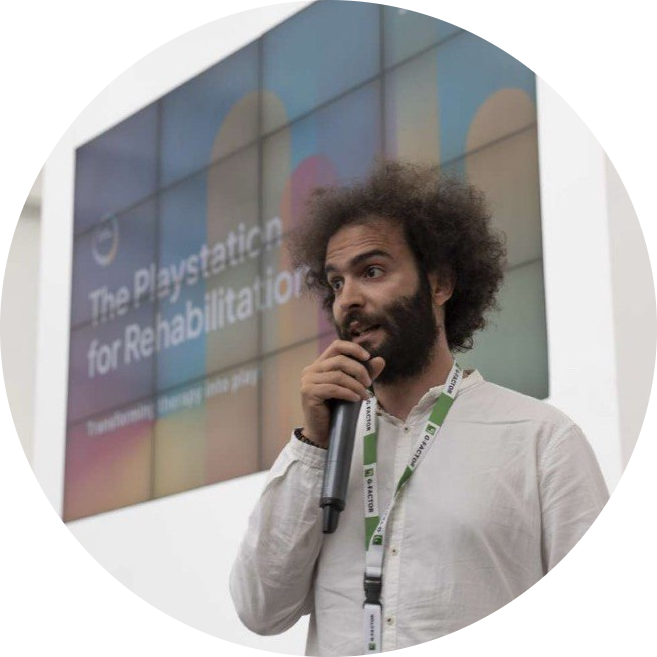
\includegraphics[width=2.8cm]{Pictures/Giovanni_pitch}
\end{minipage}
\vspace{0.1em}
}

\makeatletter
% the sender details are already in \clheader, so skip moderncv's own block
\@detailsfalse
% closing phrase, signature, name
\renewcommand*{\makeletterclosing}{%
  \@closing\\[0.6em]%
  
\includegraphics[height=1.2cm]{Pictures/sign_gt.jpg}\\[0.2em]%
  {\bfseries\@firstname~\@lastname}}
\makeatother


\begin{document}

\clheader{R\&D Engineer, PhD Candidate | Digital Health Applications}

\recipient{Talent Acquisition Team}{EUROPEAN DYNAMICS}
\opening{Dear Hiring Team,}
\closing{Yours faithfully,}
\makelettertitle

I am applying for the position of Health Applications R\&D Manager (reference HE/10/26). For more than five years I have developed health technology within publicly funded research programmes at CNR-STIIMA, the Italian National Research Council, and I would like to bring this experience to the European projects of EUROPEAN DYNAMICS.

My work covers the areas named in your vacancy: patient engagement, gamification, virtual and augmented reality, UX and IoT. In Fit4MedRob, a national programme funded by the Italian Ministry of University and Research, I defined hardware and software requirements with clinicians and deployed PhiCube rehabilitation devices in Italian clinics. In Giocabile, funded by Fondazione Cariplo, I designed the user interface and a serious game for children with cerebral palsy. I also developed an IoT multisensory feedback system for a VR/AR autism therapy platform (V.I.T.A.) and worked on driving and wheelchair VR simulators in Unity for INAIL.

Alongside research, I am co-founder and Head of Product of Rehabilia Technologies, where I lead product development with engineering, design and clinical teams, from user research to validation. PhiCube, covered by a patent of which I am co-inventor (WO2023214349A1), was validated with 19 children (SUS 85.8/100) and is now in two ongoing multicentre studies with 134 patients. We were selected for the EIT Health MedTech Bootcamp and the EIT Wildcards Bootcamp, the European support programmes for medical startups.

I am completing a PhD in Mechanics and Advanced Engineering Sciences at the University of Bologna (expected 2027). My project, OmniTrack, is an IoT-based multimodal navigation system that I built end to end, from firmware to data analysis in Python, and validated with 16 blind participants, with research stays at Utrecht University and Toyo University in Tokyo. I work in English every day, in international and multidisciplinary teams.

I would welcome the chance to discuss how I can contribute to your health projects.

\makeletterclosing

\end{document}
